\chapter{Οδηγός Χρήσης Design Pattern Builder}
\label{ch:manual}


\section{Λειτουργίες χρήστη}
\label{sec:manual}
Για να έχει τη δυνατότητα ένας προγραμματιστής να χρησιμοποιήσει το Design Pattern Builder, θα χρειαστεί:
\begin{enumerate}
    \item Να επιλέξει το πακέτο που επιθυμεί 
        ή το τρέχων έργο στο οποίο εργάζεται. 
    \item Να κάνει δεξί κλικ.
    \item Να επιλέξει New και στην καρτέλα 
        Other θα βρει την επιλογή Design Pattern Builder.
\end{enumerate} 
όπως φαίνεται στην εικόνα \ref{fig:open_wizard}, 
αφού επιλέξει Import Pattern θα εμφανιστεί ο οδηγός της εικόνας \ref{fig:select_pattern}.
\begin{figure}[H]
    \centering
    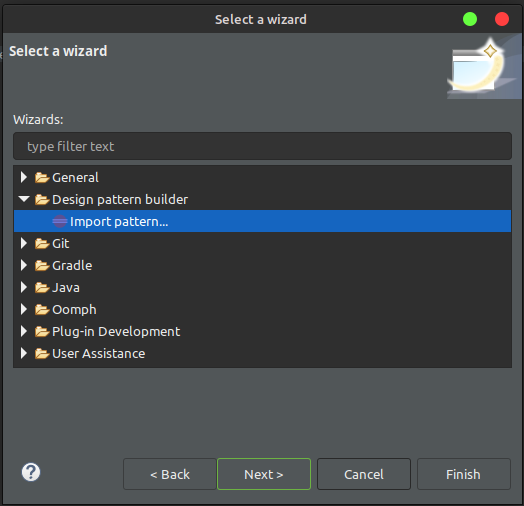
\includegraphics[width=1.0\textwidth]{Figures/open_wizard.png}
    \caption{Άνοιγμα οδηγού.}
    \label{fig:open_wizard}
\end{figure}
\begin{figure}[H]
    \centering
    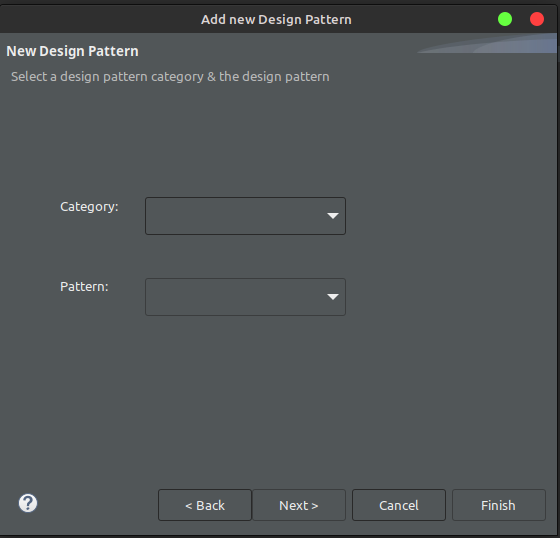
\includegraphics[width=1.0\textwidth]{Figures/select_pattern.png}
    \caption{Σελίδα επιλογής κατηγορίας \& μοτίβου.}
    \label{fig:select_pattern}
\end{figure}
Στη συνέχεια, ο προγραμματιστής έχει την δυνατότητα να επιλέξει κατηγορία μοτίβου. Αφού επιλέξει κατηγορία, τότε 
θα γίνει διαθέσιμη και η επιλογή μοτίβου. Μόλις επιλέξει και μοτίβο, τότε θα μπορεί να πλοηγηθεί στην επόμενη σελίδα του οδηγού. 
Όπως φαίνεται στην εικόνα \ref{fig:select_pattern1}.
\begin{figure}[H]
    \centering
    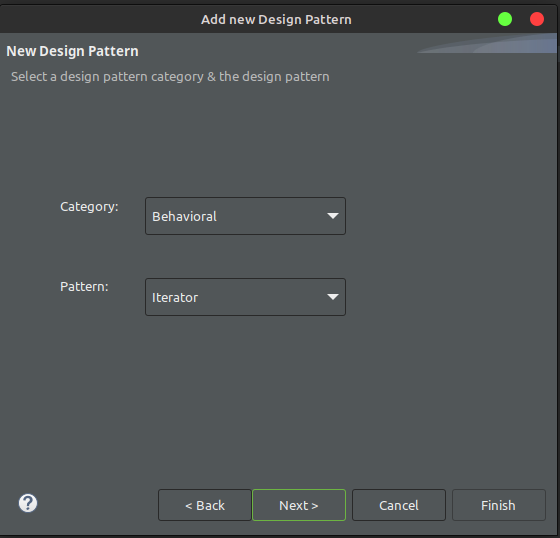
\includegraphics[width=1.0\textwidth]{Figures/select_pattern1.png}
    \caption{Επιλογή μοτίβου.}
    \label{fig:select_pattern1}
\end{figure}
Μόλις επιλέξει μοτίβο, ο οδηγός εμφανίζει τις κλάσεις και τις διεπαφές του μοτίβου. Στην εικόνα \ref{fig:classes_interfaces}, 
βλέπουμε ένα παράδειγμα για το μοτίβο Iterator \cite{GoF}. Στη συνέχεια, ο προγραμματιστής
έχει την δυνατότητα, είτε να επεξεργαστεί κάποια κλάση ή διεπαφή, επιλέγοντας την από την λίστα και κάνοντας κλικ στο αντίστοιχο κουμπί, 
είτε να προσθέσει νέα κλάση, εάν αυτό είναι επιτρεπτό, είτε να ολοκληρώσει την διαδικασία χωρίς καμία τροποποίηση 
του μοτίβου κάνοντας κλικ στο κουμπί Finish.
\begin{figure}[H]
    \centering
    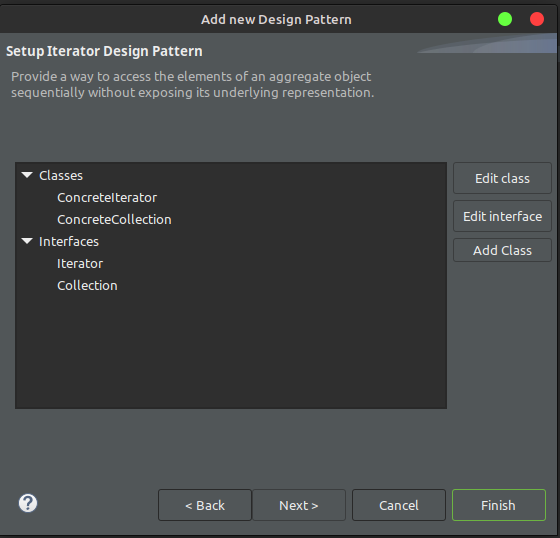
\includegraphics[width=1.0\textwidth]{Figures/classes_interfaces.png}
    \caption{Οι κλάσεις \& διεπαφές του μοτίβου Iterator.}
    \label{fig:classes_interfaces}
\end{figure}
Αφού ο προγραμματιστής επιλέξει κάποια κλάση για να επεξεργαστεί, το σύστημα θα του εμφανίσει τη σελιδά \ref{fig:class_name}, 
όπου μπορεί να αλλάξει το όνομα της κλάσης. Εάν πρόκειται για κλάση που έχει εισάγει ο χρήστης, 
να επιλέξει κάποια διεπαφή από τις διαθέσιμες για να υλοποιεί αυτή η κλάση. Επίσης, μπορεί να σταματήσει εδώ την επεξεργασία της κλάσης, 
κάνοντας κλικ στο κουμπί Finish.
\begin{figure}[H]
    \centering
    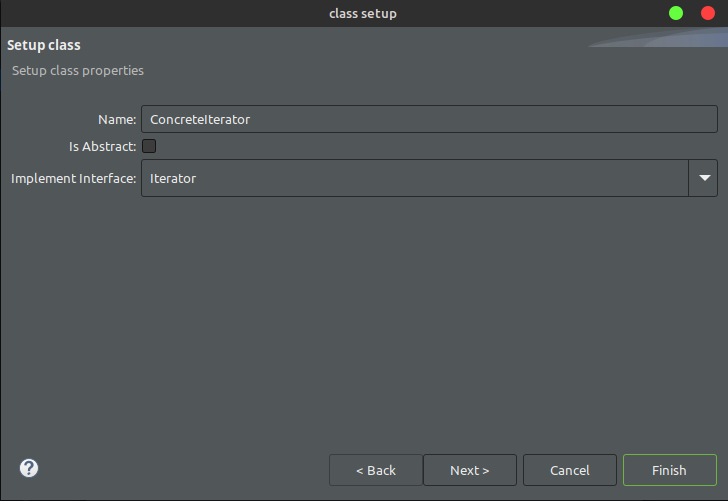
\includegraphics[width=1.0\textwidth]{Figures/class_name.png}
    \caption{Επεξεργασία ονόματος κλάσης.}
    \label{fig:class_name}
\end{figure}
Αφού έχει τροποποιήσει το όνομα της κλάσης, τότε στην επόμενη σελίδα \ref{fig:edit_fields}, 
έχει την δυνατότητα να τροποποιήσει τα πεδία της κλάσης. Αυτό επιτυγχάνεται αλλάζοντας τις τιμές στα πεδία εισόδου. 
Επίσης, μπορεί να προσθέσει ή να διαγράψει κάποιο πεδίο όπως φαίνεται στην εικόνα \ref{fig:add_field}.
\begin{figure}[H]
    \centering
    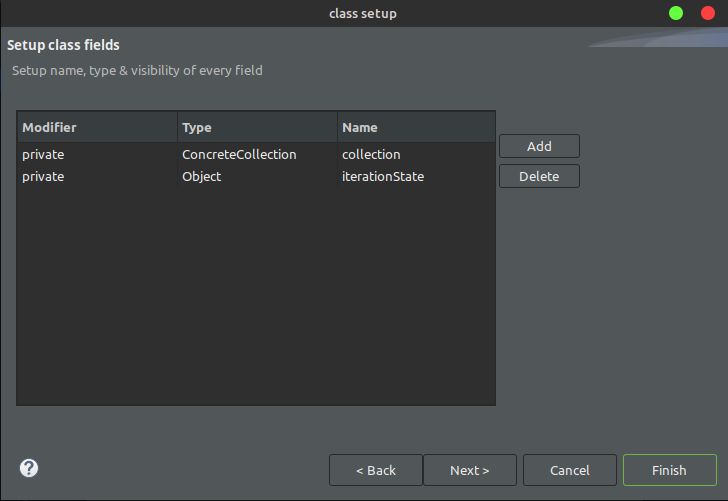
\includegraphics[width=1.0\textwidth]{Figures/edit_fields.png}
    \caption{Επεξεργασία πεδίων.}
    \label{fig:edit_fields}
\end{figure}
\begin{figure}[H]
    \centering
    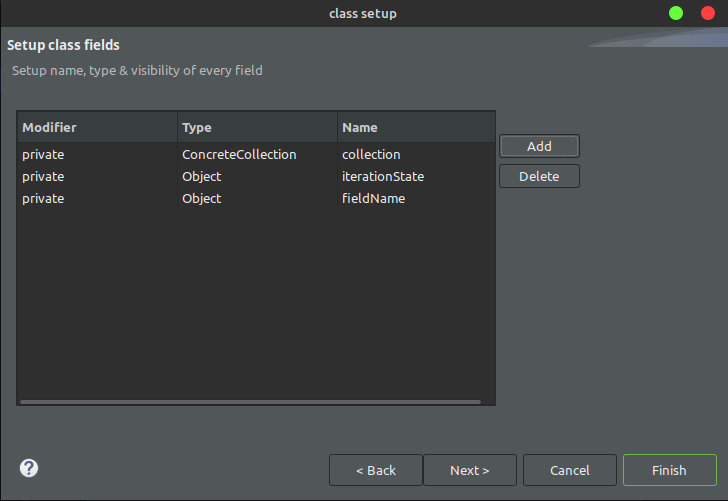
\includegraphics[width=1.0\textwidth]{Figures/add_field.png}
    \caption{Προσθήκη πεδίου.}
    \label{fig:add_field}
\end{figure}
Αφότου ο προγραμματιστής ολοκληρώσει την επεξεργασία των πεδίων, 
έχει την δυνατότητα να σταματήσει την επεξεργασία της κλάσης κάνοντας κλικ στο κουμπί finish 
ή να συνεχίσει με την επεξεργασία των μεθόδων της κλάσης. Το σύστημα θα εμφανίσει την σελίδα \ref{fig:edit_class_methods}, 
όπου φαίνονται οι μέθοδοι της κλάσης που επεξεργάζεται ο προγραμματιστής. Δίνεται η δυνατότητα να τροποποιήσει κάποια μέθοδο, 
συμπληρώνοντας τα πεδία κειμένου. Επίσης, μπορεί να προσθαφαιρέσει κάποια μέθοδο, όπως φαίνεται στην εικόνα \ref{fig:add_method}.
Τέλος, μπορεί ο προγραμματιστής να επεξεργαστεί τις παραμέτρους κάποιας μεθόδου κάνοντας κλικ στο κουμπί Edit Parameters.
\begin{figure}[H]
    \centering
    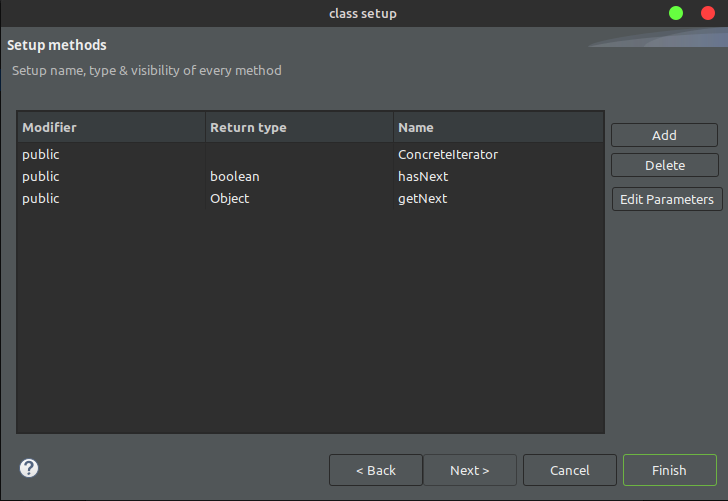
\includegraphics[width=1.0\textwidth]{Figures/edit_class_methods.png}
    \caption{Επεξεργασία μεθόδων κλάσης.}
    \label{fig:edit_class_methods}
\end{figure}
\begin{figure}[H]
    \centering
    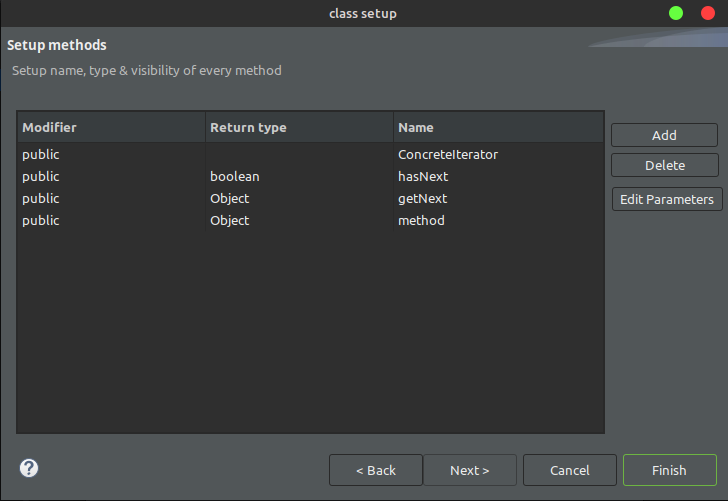
\includegraphics[width=1.0\textwidth]{Figures/add_method.png}
    \caption{Προσθήκη μεθόδου.}
    \label{fig:add_method}
\end{figure}
Μόλις ο προγραμματιστής πατήσει το κουμπί Edit Parameters, εμφανίζεται η σελίδα της εικόνας \ref{fig:edit_parameters}. 
Ο χρήστης μπορεί να προσθαφαιρέσει παραμέτρους, όπως στην εικόνα \ref{fig:add_parameters}, καθώς και να τις επεξεργαστεί.
\begin{figure}[H]
    \centering
    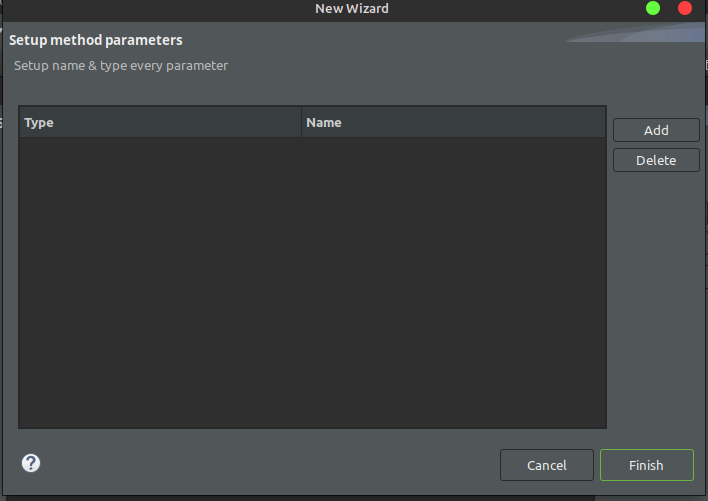
\includegraphics[width=1.0\textwidth]{Figures/edit_parameters.png}
    \caption{Επεξεργασία παραμέτρων μεθόδου.}
    \label{fig:edit_parameters}
\end{figure}
\begin{figure}[H]
    \centering
    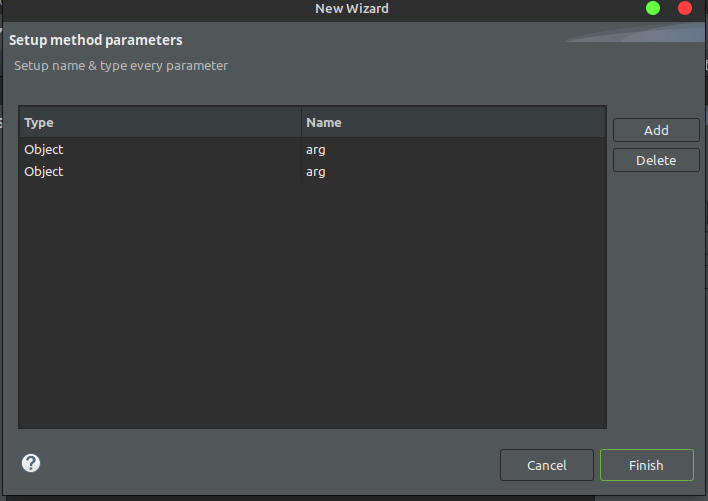
\includegraphics[width=1.0\textwidth]{Figures/add_parameters.png}
    \caption{Προσθήκη παραμέτρου.}
    \label{fig:add_parameters}
\end{figure}
Με αντίστοιχο τρόπο, ο προγραμματιστής έχει την δυνατότητα να τροποποιήσει κάποια διεπαφή του μοτίβου, 
επιλέγοντας την διεπαφή που επιθυμεί και πατώντας το κουμπί Edit interface. Εμφανίζεται ένας αντίστοιχος οδηγός, ο οποίος φαίνεται 
στην εικόνα \ref{fig:edit_interface}. Εδώ, ο προγραμματιστής δύναται να τροποποιήσει το όνομα της διεπαφής 
και να επιλέξει να τερματίσει την υπόλοιπη διαδικασία για την επεξεργασία της διεπαφής πατώντας το Finish ή να συνεχίσει στην επόμενη 
σελίδα. Η επόμενη σελίδα απεικονίζεται στην εικόνα \ref{fig:edit_interface_methods}, στην οποία μπορεί να 
επεξεργαστεί τις μεθόδους της διεπαφής, όπως ακριβώς έκανε και με κάποια κλάση.
\begin{figure}[H]
    \centering
    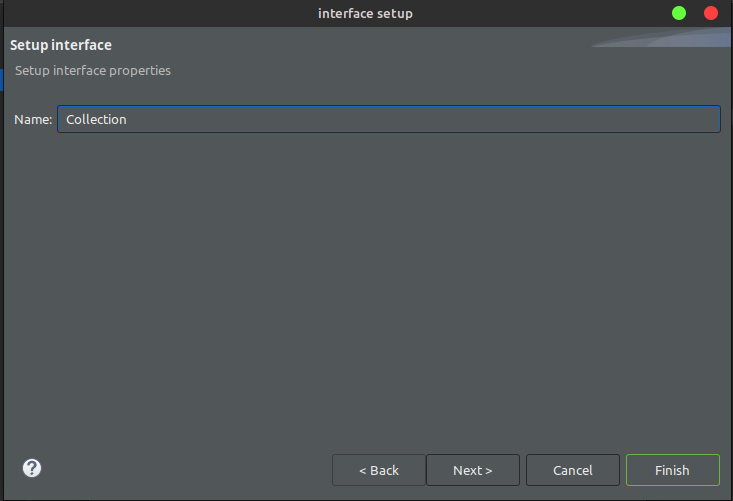
\includegraphics[width=1.0\textwidth]{Figures/edit_interface.png}
    \caption{Επεξεργασία ονόματος διεπαφής.}
    \label{fig:edit_interface}
\end{figure}
\begin{figure}[H]
    \centering
    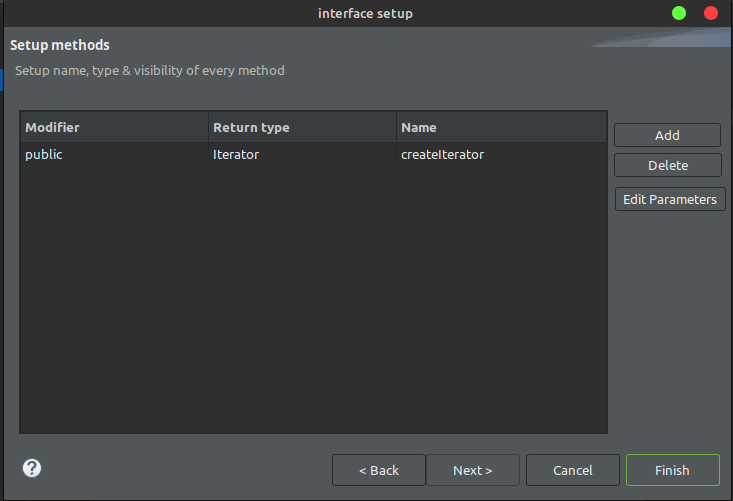
\includegraphics[width=1.0\textwidth]{Figures/edit_interface_methods.png}
    \caption{Επεξεργασία μεθόδων διεπαφής.}
    \label{fig:edit_interface_methods}
\end{figure}
Τέλος, μόλις ο προγραμματιστής κάνει τις αλλαγές που επιθυμεί, χρειάζεται να πατήσει το κουμπί Finish 
στην οθόνη \ref{fig:classes_interfaces} και το εργαλείο θα παράξει τα πηγαία αρχεία (\ref{fig:collection}, \ref{fig:concreteCollection}, \ref{fig:iterator}, \ref{fig:concreteIterator}) 
που αντιστοιχούν στο μοτίβο. 
Ο προγραμματιστής έχει την δυνατότητα να ακυρώσει και να τερματίσει τον οδηγό, οποιαδήποτε στιγμή επιθυμεί, πατώντας τα κουμπιά Cancel.
\begin{figure}[H]
    \centering
    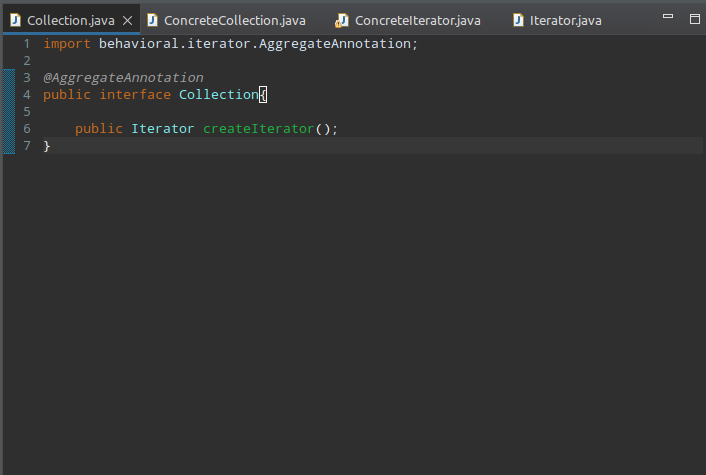
\includegraphics[width=1.0\textwidth]{Figures/collection.png}
    \caption{Διεπαφή Collection.}
    \label{fig:collection}
\end{figure}
\begin{figure}[H]
    \centering
    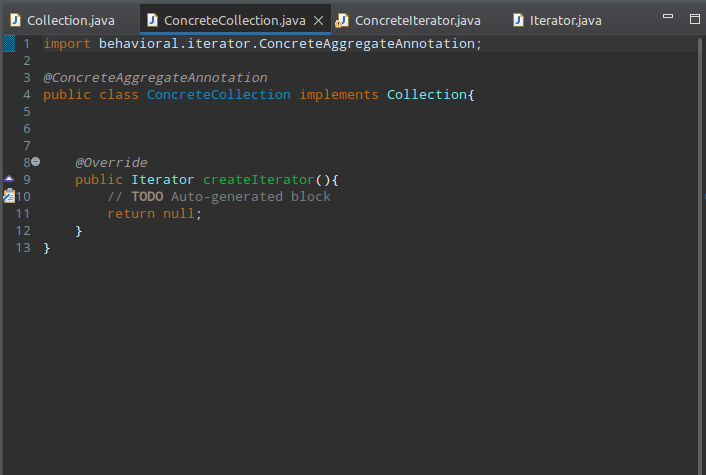
\includegraphics[width=1.0\textwidth]{Figures/concreteCollection.png}
    \caption{Κλάση ConcreteCollection.}
    \label{fig:concreteCollection}
\end{figure}
\begin{figure}[H]
    \centering
    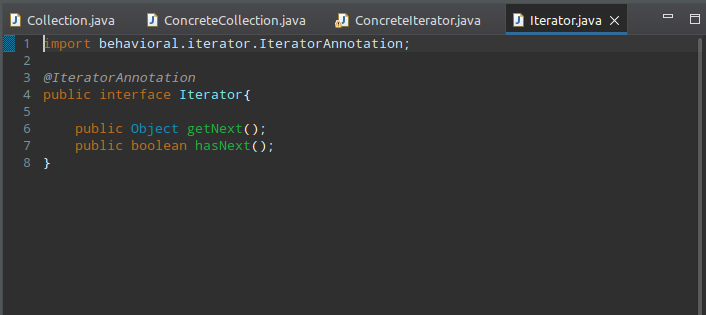
\includegraphics[width=1.0\textwidth]{Figures/iterator.png}
    \caption{Διεπαφή Iterator.}
    \label{fig:iterator}
\end{figure}
\begin{figure}[H]
    \centering
    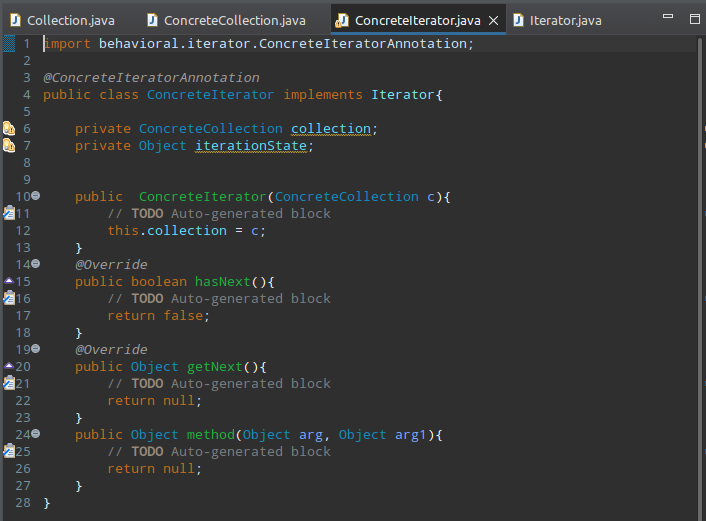
\includegraphics[width=1.0\textwidth]{Figures/concreteIterator.png}
    \caption{Κλάση ConcreteIterator.}
    \label{fig:concreteIterator}
\end{figure}